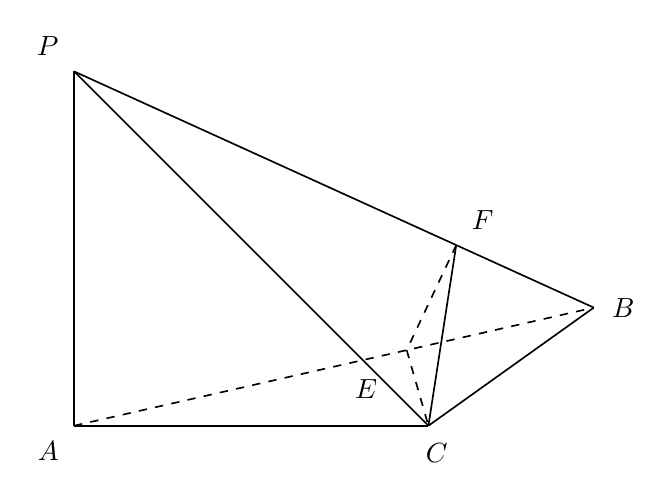
\begin{tikzpicture}[x=1cm,y=1cm,line width=.6pt,font=\normalsize]
% Tetrahedron P-ABC; F on PB and E on AB.
\coordinate (P) at (0,4.5);
\coordinate (A) at (0,0);
\coordinate (C) at (4.5,0);
\coordinate (B) at (6.6,1.5);
\coordinate (F) at (4.8529411765,2.2941176471);
\coordinate (E) at (4.2240000000,0.9600000000);
% solid visible edges
\draw (P) -- (A);
\draw (A) -- (C);
\draw (C) -- (B);
\draw (P) -- (F) -- (B);
\draw (P) -- (C);
\draw (F) -- (C);
% hidden / interior dashed edges
\draw[dashed] (A) -- (E) -- (B);
\draw[dashed] (F) -- (E);
\draw[dashed] (E) -- (C);

% labels offset from strokes
\node[above left,xshift=-2pt,yshift=2pt] at (P) {$P$};
\node[below left,xshift=-2pt,yshift=-2pt] at (A) {$A$};
\node[below,xshift=3pt,yshift=-3pt] at (C) {$C$};
\node[right,xshift=3pt] at (B) {$B$};
\node[above right,xshift=2pt,yshift=2pt] at (F) {$F$};
\node[below left,xshift=-7pt,yshift=-7pt] at (E) {$E$};
\end{tikzpicture}
